
We use cycles of execution time as a predicted output representative of application performance.  To help correlate application performance with resource utilization and not just resource allocation we also collect data from several performance counters that are usually strongly correlated with performance. These utilization metrics include L2 cache misses, L2 cache requests, and instructions retired. Any metric of interest that is measurable at runtime can be a potential output candidate. All of these models can be referenced by the spatial resource scheduling algorithm.


A final model we create predicts the energy consumed by a resource allocation, which is useful  for energy-aware scheduling decisions. We calculate the energy used by each allocation by creating a simple energy model which incorporates energy levels for allocated versus unallocated resources and uses performance counter data as a proxy for resource activity.  Such an energy model is clearly somewhat simplistic --- we include it to show that our scheduling framework can feasibly make decisions based on per allocation energy if that data is a given input.  We use a simplified version of some of the activity based energy models in previous work \cite{}.

We perform this analysis for several performance metrics captured from simulation, including runtime in cycles, number of instructions committed, number of cache accesses, and number of off-chip memory accesses.

\begin{table}
\scriptsize
\begin{tabular}{|l|c|c|c|}
\hline
Name & Additive & Quadratic & GPRS \\ \hline
  p--c--b-- & 392.11\% (398.89) &  240.12\% (261.72) & 7.42\% (16.80)  \\ \hline
 p--c--b+ &  138133\% (290142)&  105682\% (248332) &  253.46\% (418.27)  \\ \hline
 p--c+b-- &   37225\% (65356) &  25797\% (47989) & 84.31\% (74.62)  \\ \hline
 p--c+b+ &   45276\% (82816) &  21819\% (30963) &  87.84\% (209.33)  \\ \hline
 p+c--b-- & 236.30\% (261.31) &  121.44\% (124.23) & 15.27\% (14.80)    \\ \hline
 p+c--b+ &   101696\% (169812)  &  73241\% (117426) & 25.42\% (31.95) \\ \hline
 p+c+b--&  16920\% (22871)&   12517\% (19362) & 7.47\% (8.25)  \\ \hline
 p+c+b+&   9480\% (11542) &  6647\% (9164) &  22.12\% (26.14)  \\ \hline
  \end{tabular}
 \caption{Means (standard deviations) of percentage error in offchip accesses for each of the predictive models for each of the microbenchmarks.}
\label{table:acc-offchip}
\end{table}

\begin{table}
\small
\begin{tabular}{|l|c|c|c|}
\hline
Name & Additive & Quadratic & GPRS \\ \hline
 p--c--b-- & 0.03\% (0.04) & 0.03\% (0.05) & 0.28\% (0.36) \\ \hline
 p--c--b+ & 241.91\% (262.05)  & 218.93\% (382.43) &  0.1\% (0.07) \\ \hline
 p--c+b-- & 8.49\% (5.49) & 6.17\% (6.50) & 0.41\% (1.13) \\ \hline
 p--c+b+ & 8.01\% (5.2)  & 5.79\% (6.11) & 0.07\% (0.06) \\ \hline
 p+c--b-- & 7.28\% (10.50)  & 0.05\% (0.04) & 0.27\%(0.19) \\ \hline
 p+c--b+ & 233.26\% (250.1) & 153.10\% (234.34) &  4.89\% (12.97)\\ \hline
 p+c+b-- & 20.23\% (24.18)  & 5.10\% (4.26) &  0.30\% (0.28) \\ \hline
 p+c+b+ & 13.30\% (10.23)  & 5.25\% (4.77)  & 0.05\% (0.03) \\ \hline
  \end{tabular}
 \caption{Means (standard deviations) of percentage error in cache transaction counts for each of the predictive models for each of the microbenchmarks.}
\label{table:acc-cache}
\end{table}

%\begin{table}
%\small
%\begin{tabular}{|l|c|c|c|}
%\hline
%Name & Cycles &Offchip Accesses &Cache Accesses \\ \hline
% p--c--b-- & 0.06\% (0.04) &  392.11\% (398.89) & 0.03\% (0.04) \\ \hline
% p--c--b+ &   234.07\% (287.44) & 138133\% (290142) & 241.91\% (262.05)  \\ \hline
% p--c+b-- &  12.67\% (5.30) & 37225\% (65356) & 8.49\% (5.49)  \\ \hline
% p--c+b+ &  12.04\% (5.09) &  45276\% (82816) & 8.01\% (5.2)  \\ \hline
% p+c--b-- &  0.07\% (0.05) &  236.30\% (261.31) & 7.28\% (10.50)  \\ \hline
% p+c--b+ &  271.05\% (377.53) & 101696\% (169812) & 233.26\% (250.1)  \\ \hline
% p+c+b--&  13.08\% (6.91) & 16920\% (22871) & 20.23\% (24.18)  \\ \hline
% p+c+b+&  12.07\% (4.86) &  9480\% (11542) & 13.30\% (10.23)  \\ \hline \hline
% cluster &  1 (1) & 1 (1)  & 1 (1)  \\ \hline
% gaussian&  1 (1) & 1 (1) & 1 (1)  \\ \hline
% update&  1 (1) & 1 (1)  & 1 (1)  \\ \hline
% pruning&  1 (1) & 1 (1)  & 1 (1)  \\ \hline
% epsilon &  1 (1) & 1 (1)  & 1 (1)  \\ \hline
% \end{tabular}
% \caption{Means (standard deviations) of percentage error for each of the performance measures for each of the benchmarks, as predicted by the linear response surface model.}
%\label{table:acc-lin}
%\end{table}
%
%\begin{table}
%\small
%\begin{tabular}{|l|c|c|c|}
%\hline
%Name & Cycles &Offchip Accesses &Cache Accesses \\ \hline
% p--c--b-- & 0.04\% (0.04) &  240.12\% (261.72) & 0.03\% (0.05) \\ \hline
% p--c--b+ &  139.21\% (167.10) &  105682\% (248332) & 218.93\% (382.43)  \\ \hline
% p--c+b-- &  8.26\% (5.30) &  25797\% (47989) & 6.17\% (6.50)  \\ \hline
% p--c+b+ &  7.83\% (4.69) &  21819\% (30963) & 5.79\% (6.11)  \\ \hline
% p+c--b-- &  0.05\% (0.06) &  121.44\% (124.23) & 0.05\% (0.04)  \\ \hline
% p+c--b+ &  164.23\% (226.23) &  73241\% (117426) & 153.10\% (234.34)  \\ \hline
% p+c+b--&  8.79\% (7.32) &   12517\% (19362) & 5.10\% (4.26)   \\ \hline
% p+c+b+&  8.05\% (5.49) &  6647\% (9164) & 5.25\% (4.77)  \\ \hline \hline
% cluster &  1 (1) & 1 (1) & 1 (1)  \\ \hline
% gaussian&  1 (1) & 1 (1) & 1 (1)  \\ \hline
% update&  1 (1) & 1 (1) &  1 (1)  \\ \hline
% pruning&  1 (1) & 1 (1) & 1 (1)  \\ \hline
% epsilon &  1 (1) & 1 (1) &  1 (1)  \\ \hline
% \end{tabular}
% \caption{Means (standard deviations) of percentage error for each of the performance measures for each of the benchmarks, as predicted by the quadratic response surface model.}
%\label{table:acc-quad}
%\end{table}
%
%\begin{table}
%\small
%\begin{tabular}{|l|c|c|c|}
%\hline
%Name & Cycles &Offchip Accesses &Cache Accesses \\ \hline
% p--c--b-- & 0.02\% (0.02) &   7.42\% (16.80) & 1 (1) \\ \hline
% p--c--b+ &  0.23\% (0.40) &  253.46\% (418.27) & 1 (1)  \\ \hline
% p--c+b-- &  0.02\% (0.02) &  84.31\% (74.62) & 1 (1)  \\ \hline
% p--c+b+ &  0.06\% (0.06) &  87.84\% (209.33) & 1 (1)  \\ \hline
% p+c--b-- &  0.05\% (0.03) &  15.27\% (14.80) & 1 (1)  \\ \hline
% p+c--b+ &  0.51\% (1.08) &  25.42\% (31.95) & 1 (1)  \\ \hline
% p+c+b--&  0.06\% (0.07) &  7.47\% (8.25)) & 1 (1)  \\ \hline
% p+c+b+&  0.08\% (0.06) &  22.12\% (26.14) & 1 (1)  \\ \hline \hline
% cluster &  1 (1) & 1 (1) &  1 (1)  \\ \hline
% gaussian&  1 (1) & 1 (1) & 1 (1)  \\ \hline
% update&  1 (1) & 1 (1)  & 1 (1)  \\ \hline
% pruning&  1 (1) & 1 (1) & 1 (1)  \\ \hline
% epsilon &  1 (1) & 1 (1) & 1 (1)  \\ \hline
% \end{tabular}
% \caption{Means (standard deviations) of percentage error for each of the performance measures for each of the benchmarks, as predicted by the GPRS model.}
%\label{table:acc-nonlin}
%\end{table}

Table~\ref{table:acc-offchip} does the same for the off-chip accesses metric and Table~\ref{table:acc-cache} for the L2 cache transactions metric.  Points in the test set are not in the training set.


For all benchmarks, the number of instructions was relatively easy to predict, while the off-chip bandwidth and number of cache accesses were much more difficult.  Performance (cycles) prediction accuracy fell in between.  The benchmarks with the worst standard deviations had several extreme outliers that reduced the mean accuracy. Since the accuracy reported in the aforementioned tables is {\em percentage} error, it is subject to inflation when some absolute values being predicted are small relative to others in the set, which is the case particularly for off-chip bandwidth measurements.  Therefore, our judgement of model quality is dependent on how much we value accurate prediction of these small values.  For example, the GPRS--based model of microbenchmark \texttt{  p--c--b+}'s offchip accesses has a percentage error of 253.46\%, but this is caused by mispredictons of less than 5000 accesses (versus up to 2 million accesses incurred by the benchmark for certain resource allocations).

\subsubsection*{Effect of Sample Size on Model Accuracy}
\label{sec:eval:acc-sample}

Figure ~\ref{fig:acc-sample} shows the impact that changing the sample set size has on model accuracy, using the example of execution time predictions for the microbenchmarks.  It is worth noting that while the accuracy of the quadratic and  nonlinear models improve rapidly with increasing sample size, the linear additive model sees no improvement on average.  This failure to improve when exposed to additional data indicates that it is the {\em form} of the model itself which is flawed (i.e. too simplistic).  Another important feature is that as sample size increases, the improvement seen by the other models slows, indicating a point of diminishing returns for increasing sample size.

This sample size analysis informs our decision about whether we can afford to use online or offline, linear or nonlinear models.  On the one hand, GPRS--based nonlinear models are much more accurate even when given smaller sample sizes.  However, they take a long time to train, and cannot be rapidly adapted to account for new data points.  On the other hand, linear models of sufficient complexity require more points to succeed, but can be rapidly trained and retrained.  A hybrid approach, in which genetic programming is used to construct the form of the response surface model offline, and then the model's coefficients are retuned based on performance data collected online, may a viable way to get the best of both worlds.

\begin{figure}
	\centering
	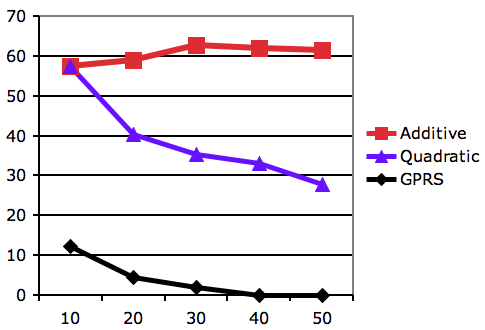
\includegraphics[scale = 0.5] {Figures/acc_sample.png}
	\caption{ \small Comparison of model accuracy for different models as training sample size is increased.  Y-axis is average percentage error in predictions of runtime averaged across all benchmarks. X-axis is increasing sample size.  Some models are more robust to reduced sample size than others.}
	\label{fig:acc-sample}
\end{figure}
